\chapter{Introduction}
\label{chap:Intro}


\section{Ultrafast Science}

Since the discovery of the laser \cite{schawlowInfraredOpticalMasers1958, maimanStimulatedOpticalRadiation1960} and the subsequent demonstration of nonlinear optics \cite{frankenGenerationOpticalHarmonics1961, armstrongInteractionsLightWaves1962}, one of the areas that has seen a great amount of interest is the use of lasers to study the dynamics of various systems.  This is generally done by taking advantage of the ability to create a pulsed laser.  This occurs when the spectral phase and amplitude of a laser coherently combines to create an intense burst of light as a function of time.  As an example, a typical approximation is to assume that the electric field $\mathcal{E}(t)$ can be written as a Gaussian, such as
\begin{equation}
	\label{eqn:gaussian_pulse}
	\mathcal{E}(t) = \mathcal{E}_0 e^{-2\ln 2(\frac{t}{\Delta t})^2}\cos(\omega_0 t + \theta(t))
\end{equation}
where $\Delta t$ is the pulse duration, $\omega_0$ is the carrier frequency, and $\theta(t)$ determines the temporal relationship between the frequency components that are within the pulse bandwidth.  An example of just such a pulse shape is shown in figure \ref{fig:gaussian_pulse} in both time and frequency, and it can be shown that the pulse duration $\Delta t$ is inversely proportional to the spectral bandwidth $\Delta\omega$.  This entails that larger bandwidths are required to achieve shorter transform limited pulse durations.

The need for shorter duration pulses is shown in figure \ref{fig:Pulse_duration}.


\begin{figure}
	\centering
	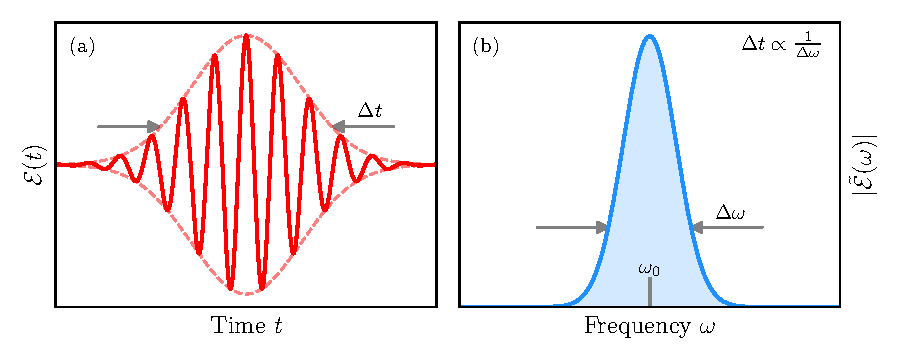
\includegraphics[width=1.0\textwidth]{figures/Introduction/gaussian_pulse.pdf}
	\caption[Example of a typical Gaussian pulse in time and frequency]{Example of a typical Gaussian pulse in time (a) and frequency (b).  The pulse duration $\Delta t$ and the spectral bandwidth $\Delta\omega$ are shown, as well as the relationship between them.}
	\label{fig:gaussian_pulse}
\end{figure}

\begin{figure}
	\centering
	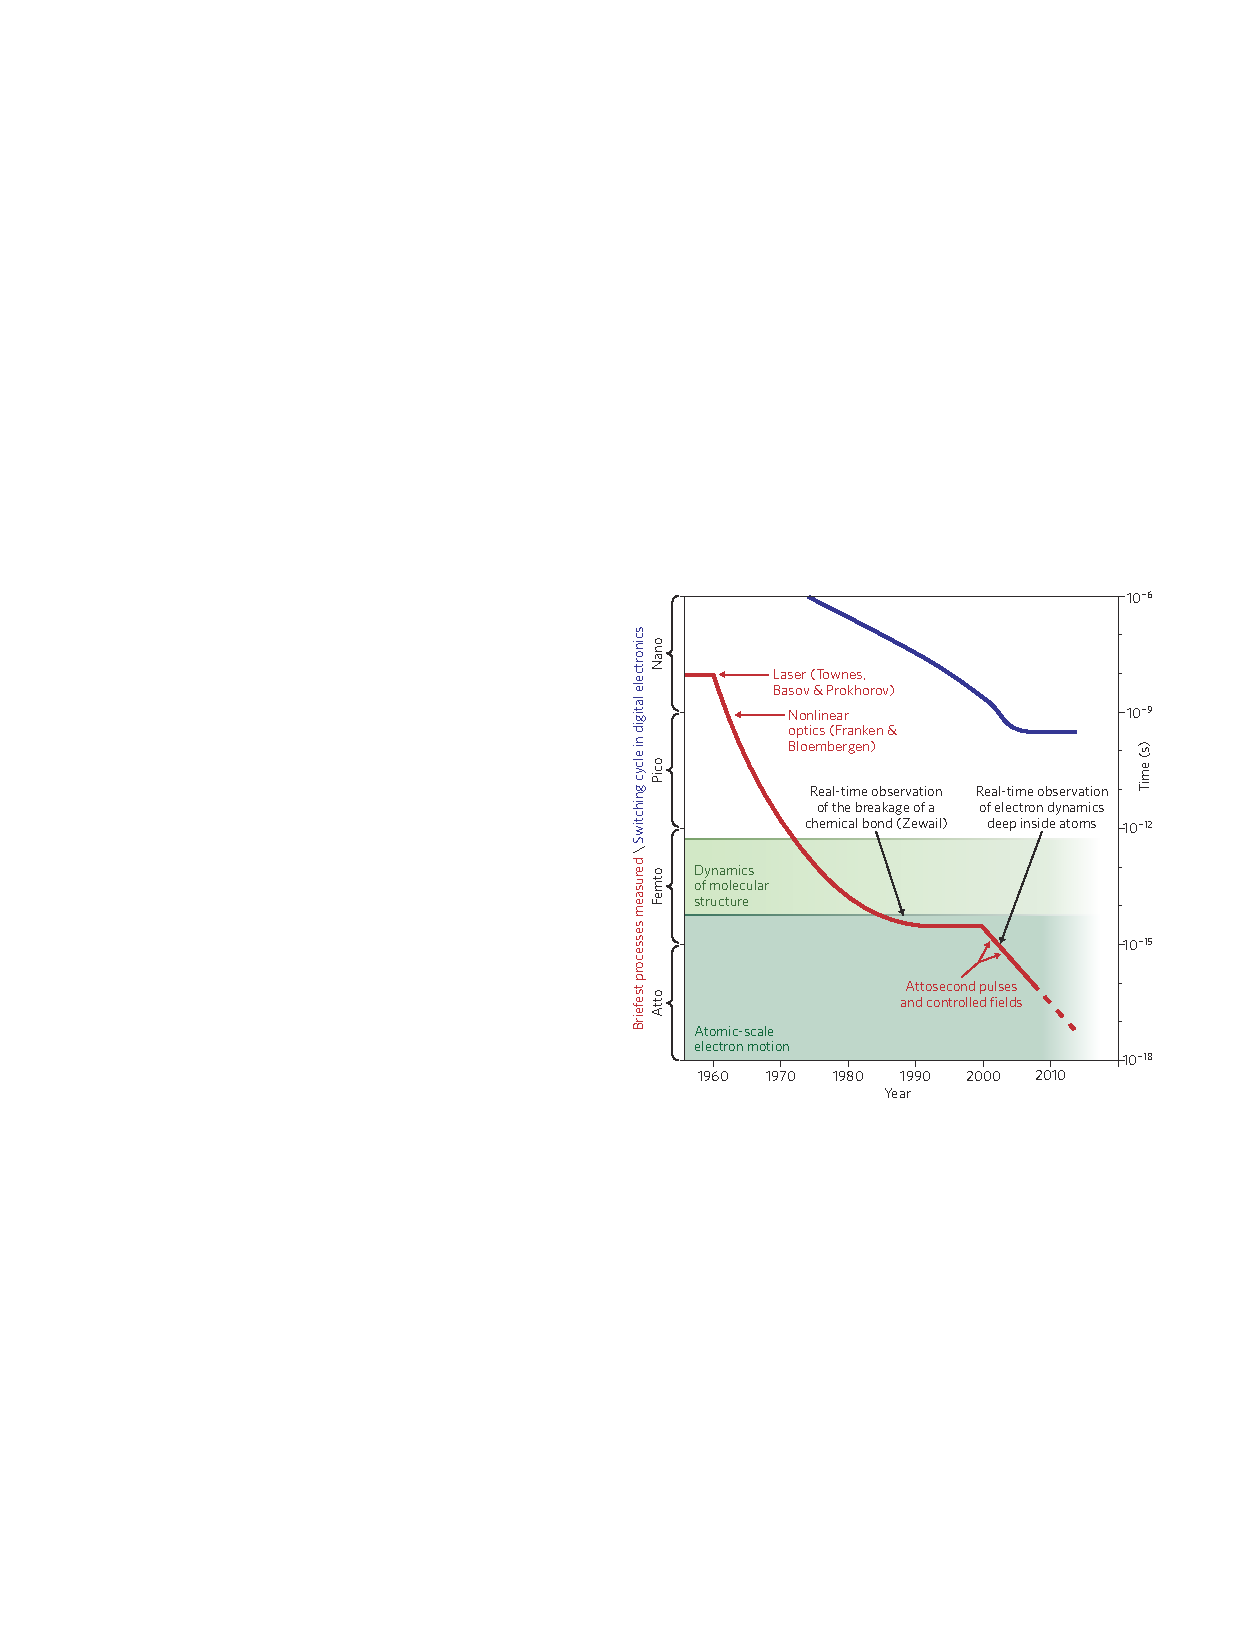
\includegraphics[width=0.5\textwidth]{figures/Introduction/Pulse_duration.pdf}
	\caption[Recollision model of high harmonic generation]{Recollision model of high harmonic generation.  The three steps are (1) tunnel ionization, (2) propagation/acceleration in the laser field, and (3) recombination and photoemission.}
	\label{fig:Pulse_duration}
\end{figure}

\section{High-Harmonic Generation}
\label{intro_HHG}

\begin{figure}
	\centering
	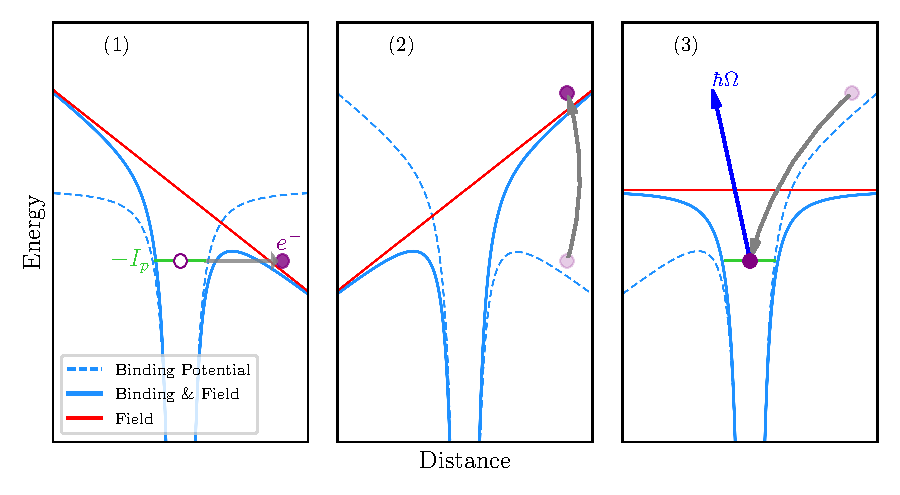
\includegraphics[width=1.0\textwidth]{figures/Introduction/3-step.pdf}
	\caption[Recollision model of high harmonic generation]{Recollision model of high harmonic generation.  The three steps are (1) tunnel ionization, (2) propagation/accelaration in the laser field, and (3) recombination and photoemission.}
	\label{fig:3-step}
\end{figure}

\begin{figure}
	\centering
	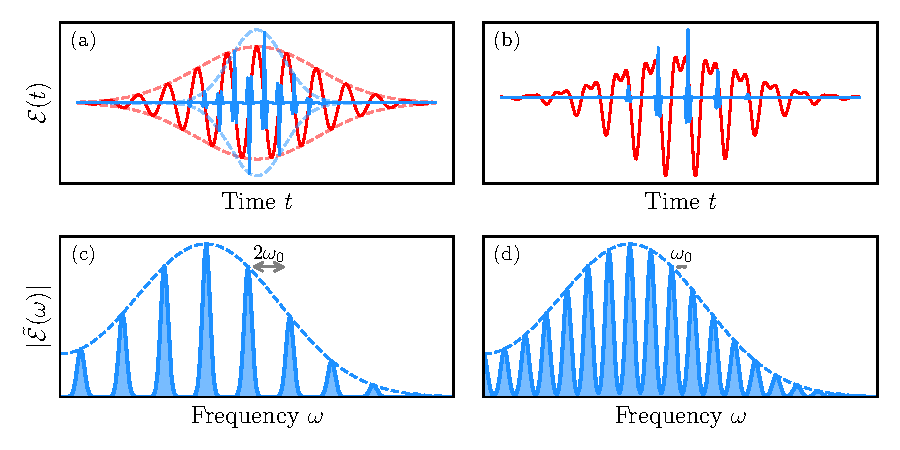
\includegraphics[width=1.0\textwidth]{figures/Introduction/time_to_freq.pdf}
	\caption[Example electric field of XUV APT and its frequency spectrum]{(a) Example of the electric field of an XUV APT.  There is a burst every half-cycle of the fundamental field period $\tau_0$.  (b)  Spectral amplitude of APT.  Harmonics are separated by $2\omega_0=4\pi/\tau_0$.  Bandwidth of each harmonic is determined by the number of cycles in the fundamental pulse, and the overall bandwidth is determined by the pulse duration of each burst in the train. (b) Example of a two-color $\omega-2\omega$ fundamental field.  The asymmetry of the pulse means there is a burst once every cycle. (d) The spectral amplitude for the asymmetric field, and now there are even and odd harmonics.  The dashed line in (c) and (d) represent the spectral amplitude of just one of the pulses in the pulse train.}
	\label{fig:time_to_freq}
\end{figure}


\section{Transient Absorption Spectroscopy}
\label{into_theory_cats}

\begin{figure}
	\centering
	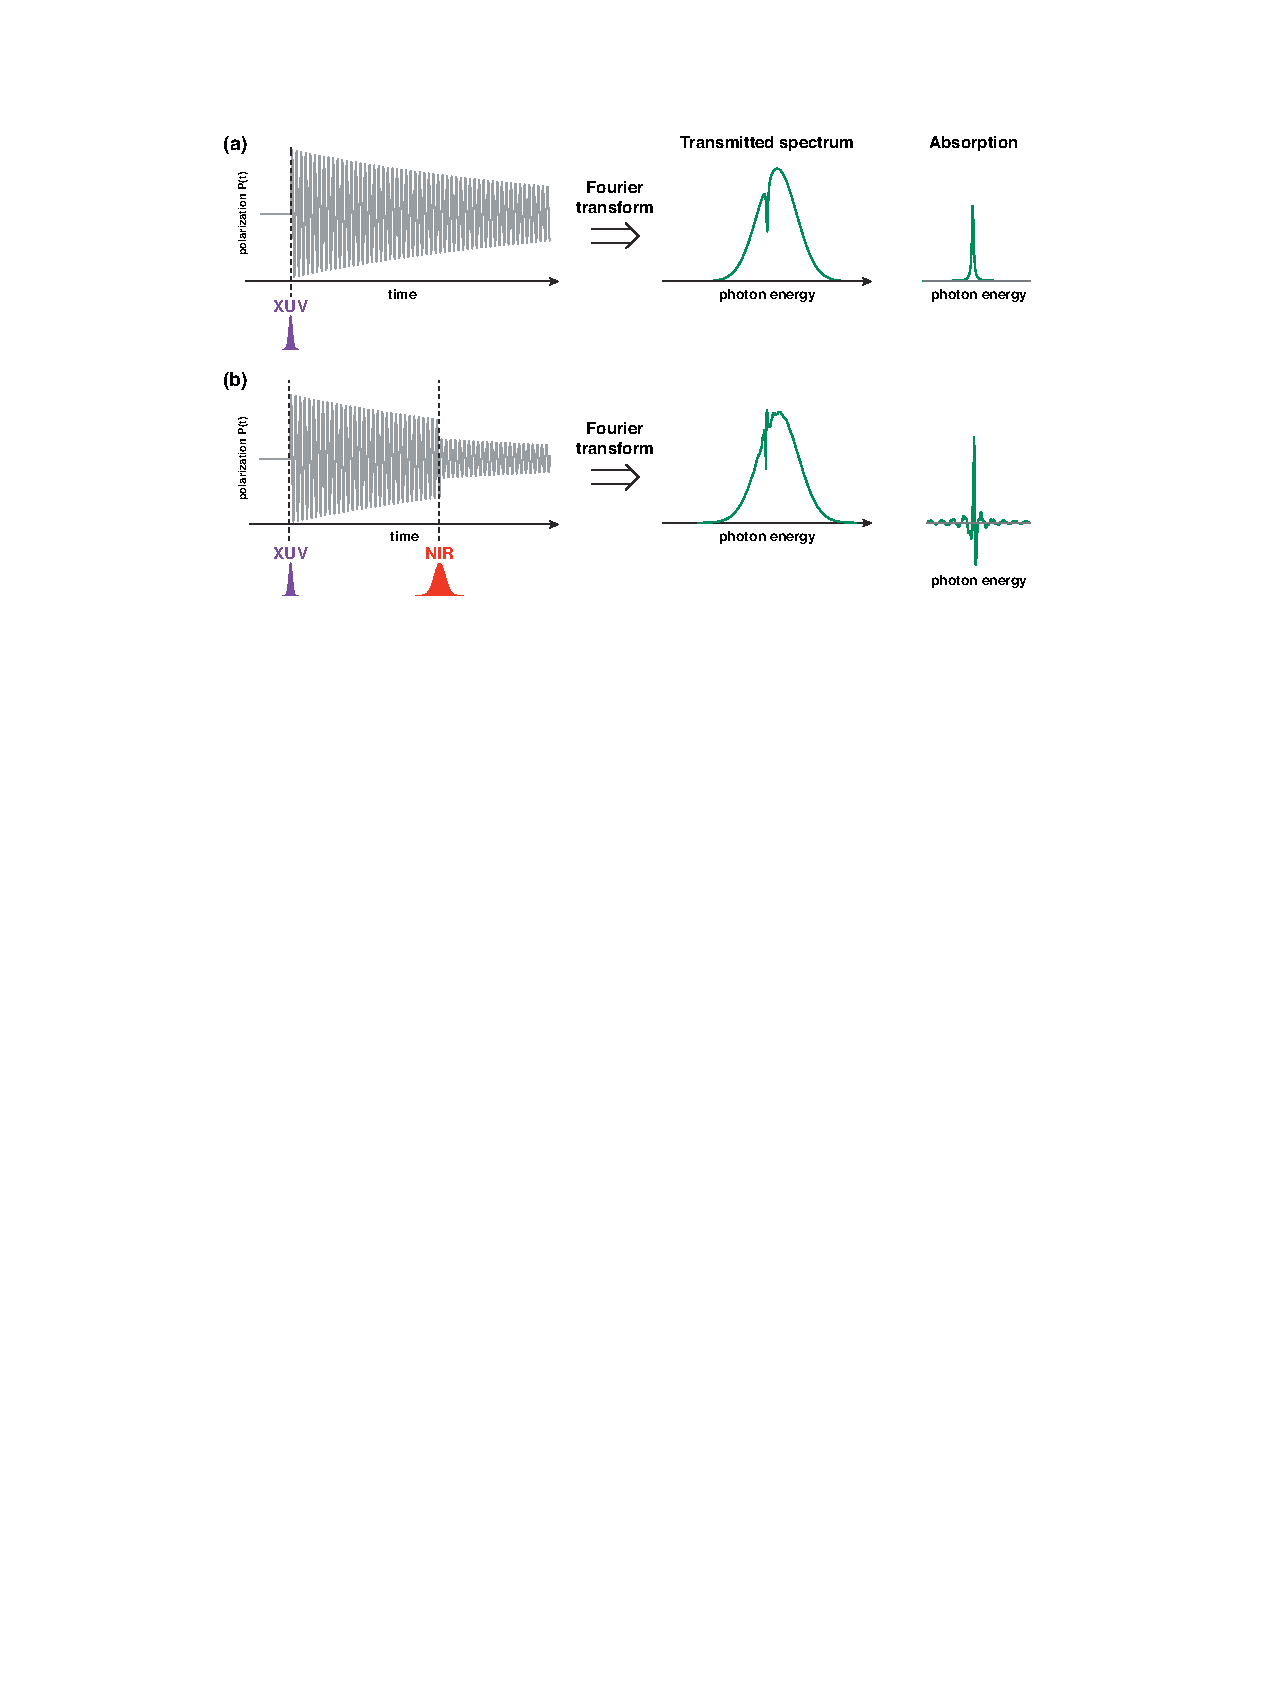
\includegraphics[width=1.0\textwidth]{figures/Introduction/gas_TA_sketch.pdf}
	\caption[Example electric field of XUV APT and its frequency spectrum]{(a) Example of the electric field of an XUV APT.  There is a burst every half-cycle of the fundamental field period $\tau_0$.  (b)  Spectral amplitude of APT.  Harmonics are separated by $2\omega_0=4\pi/\tau_0$.  Bandwidth of each harmonic is determined by the number of cycles in the fundamental pulse, and the overall bandwidth is determined by the pulse duration of each burst in the train. (b) Example of a two-color $\omega-2\omega$ fundamental field.  The asymmetry of the pulse means there is a burst once every cycle. (d) The spectral amplitude for the asymmetric field, and now there are even and odd harmonics.  The dashed line in (c) and (d) represent the spectral amplitude of just one of the pulses in the pulse train.}
	\label{fig:gas_TA_sketch}
\end{figure}

